%************************************************
\chapter{The Mind Monitor Application}
\label{chapter:the_mind_monitor_application}
%************************************************

In order to control the SALS model of mind, a mind monitoring
application called \emph{MindMon} has been implemented.  MindMon is
based on abstract physical world and reflective thinking components
that allow reflective thinking layers to be interchanged with
different $\text{reflective}^0$ physical layers.  In this dissertation
I focus on a block building domain in order to demonstrate
second-order reflective learning to plan, but other more complex
physical domains have also been developed within SALS such as the
IsisWorld physical simulator described by \cite{smith:2010}, where
MindMon allows attaching multiple reflective thinking models to a
shared $\text{reflective}^0$ physical layer, a type of simulation that
assumes a more complex subjective philosophy of mind that is not
assumed in the non-subjective model described in
{\mbox{\autoref{part:the_model}}} of this thesis.
{\mbox{\autoref{figure:implemented_mindmon}}} shows the implemented
MindMon application.
\begin{figure}
\hspace*{-1cm}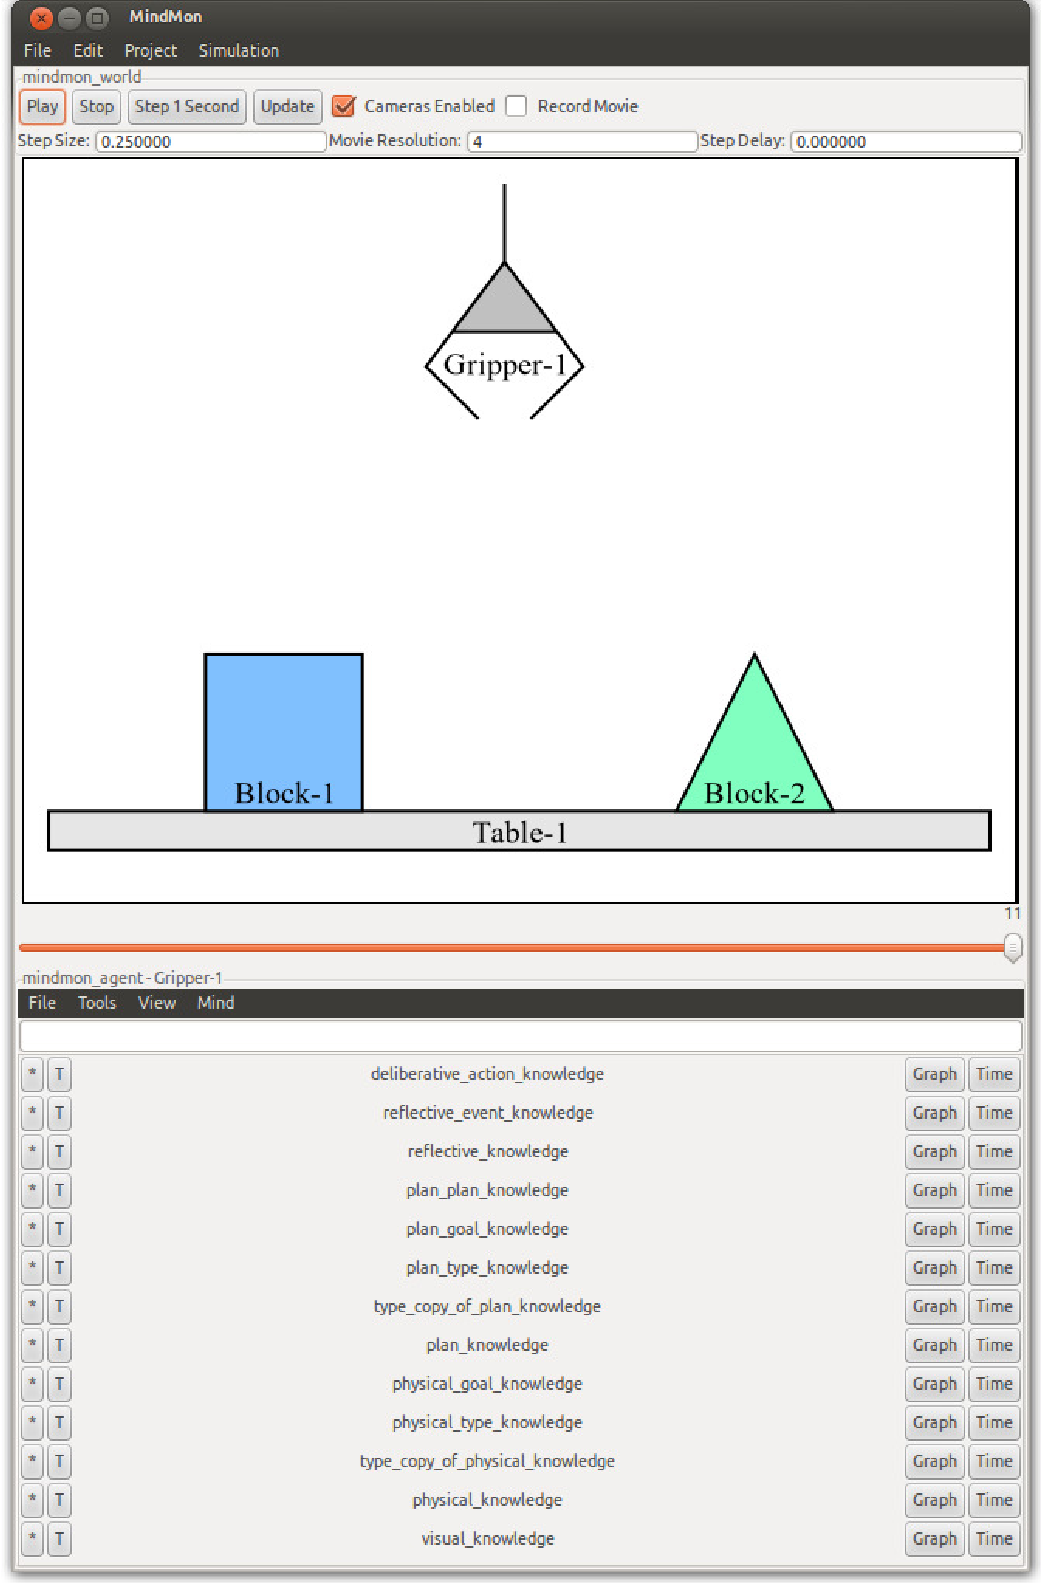
\includegraphics[width=13cm]{gfx/implemented_mindmon}
\caption[The implemented mind monitoring application, MindMon.]{The
  implemented mind monitoring application, MindMon, shown here with
  the simple block building domain and the reflective thinking layers
  described in this dissertation.}
\label{figure:implemented_mindmon}
\end{figure}

\section{The Physical Knowledge-Base}

The block building domain is a simulation based on two-dimensional
ridid-body physical laws, including floating point numerical
representations for object positions, velocities and accellerations.
These numerical representations and the processes that manipulate them
are part of the $\text{reflective}^0$ physical layer of the model, but
in order to focus the efficiency of the procedural reflection, a much
simpler relational graph representation has been specifically
represented in semantic frame-based objects in a semantic
knowledge-base, referred to as the \emph{physical knowledge-base}.
The physical knowledge-base includes objects with shapes, colors, and
multiple prepositional spatial relationships.
{\mbox{\autoref{figure:implemented_physical_knowledge}}} shows the
implemented physical knowledge.
\begin{sidewaysfigure}
\begin{center}
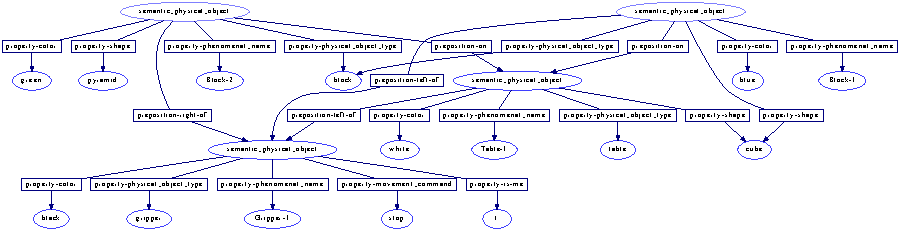
\includegraphics[width=24cm]{gfx/implemented_physical_knowledge}
\end{center}
\hspace{4cm}\parbox{15cm}{\caption[The implemented physical
    knowledge-base.]{The implemented physical
    knowledge-base.}\label{figure:implemented_physical_knowledge}}
\end{sidewaysfigure}

\section{Semantic Event Knowledge-Base}

%{\mbox{\autoref{figure:implemented_semantic_event_knowledge_base}}} shows the
%implemented semantic event knowledge base.
%\begin{figure}
%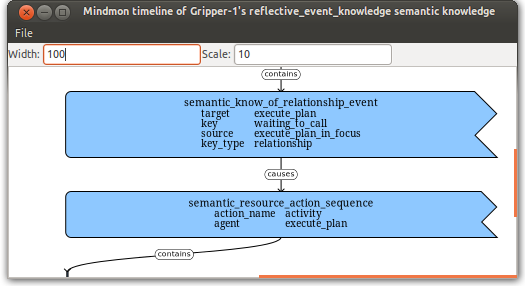
\includegraphics[width=10cm]{gfx/implemented_semantic_event_knowledge_base}
%\caption[The implemented semantic event knowledge base.]{The
%  implemented semantic event knowledge base.}
%\label{figure:implemented_semantic_event_knowledge_base}
%\end{figure}

{\mbox{\autoref{figure:implemented_reflective_event_knowledge_base}}}
shows the implemented semantic event knowledge base.
\begin{figure}
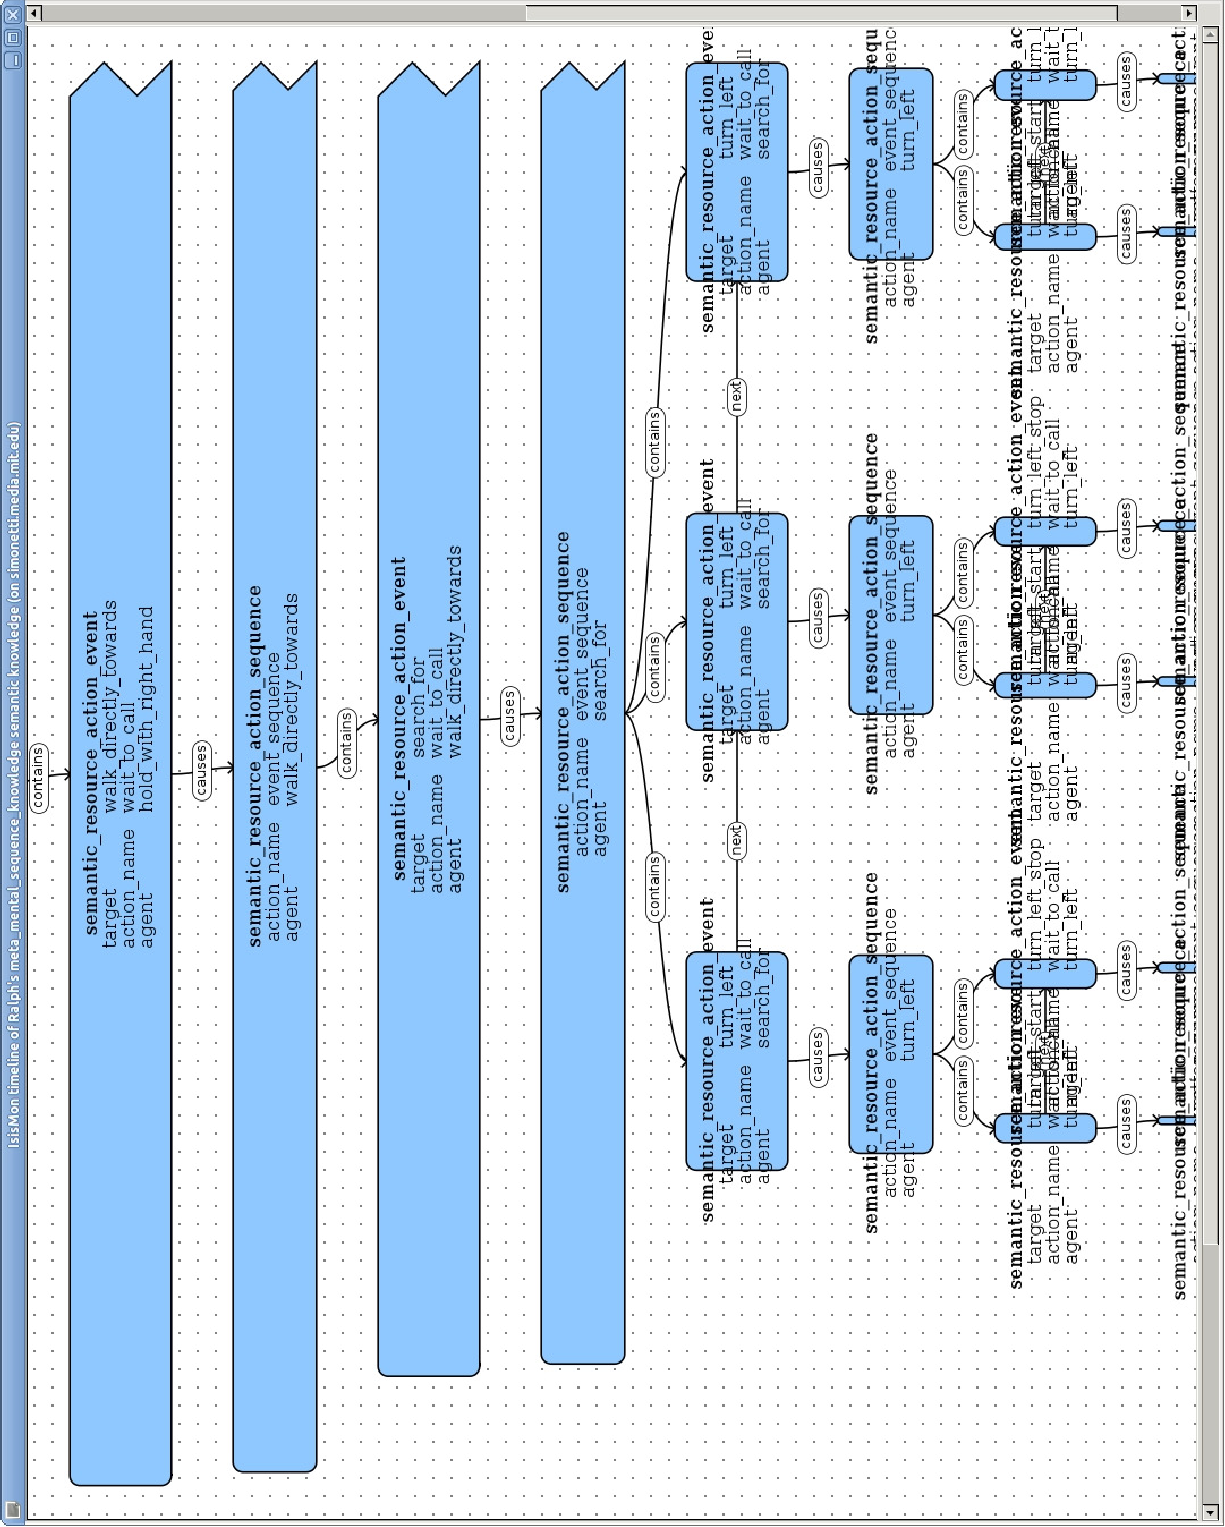
\includegraphics[width=10cm]{gfx/implemented_reflective_event_knowledge_base}
\caption[The implemented semantic event knowledge base.]{The
  implemented semantic event knowledge base.}
\label{figure:implemented_reflective_event_knowledge_base}
\end{figure}

%\section{IsisWorld First-order Resource Activator}

%{\mbox{\autoref{figure:implemented_isisworld_first_order_resource_activator}}}
%shows the implemented semantic event knowledge base.
%\begin{figure}
%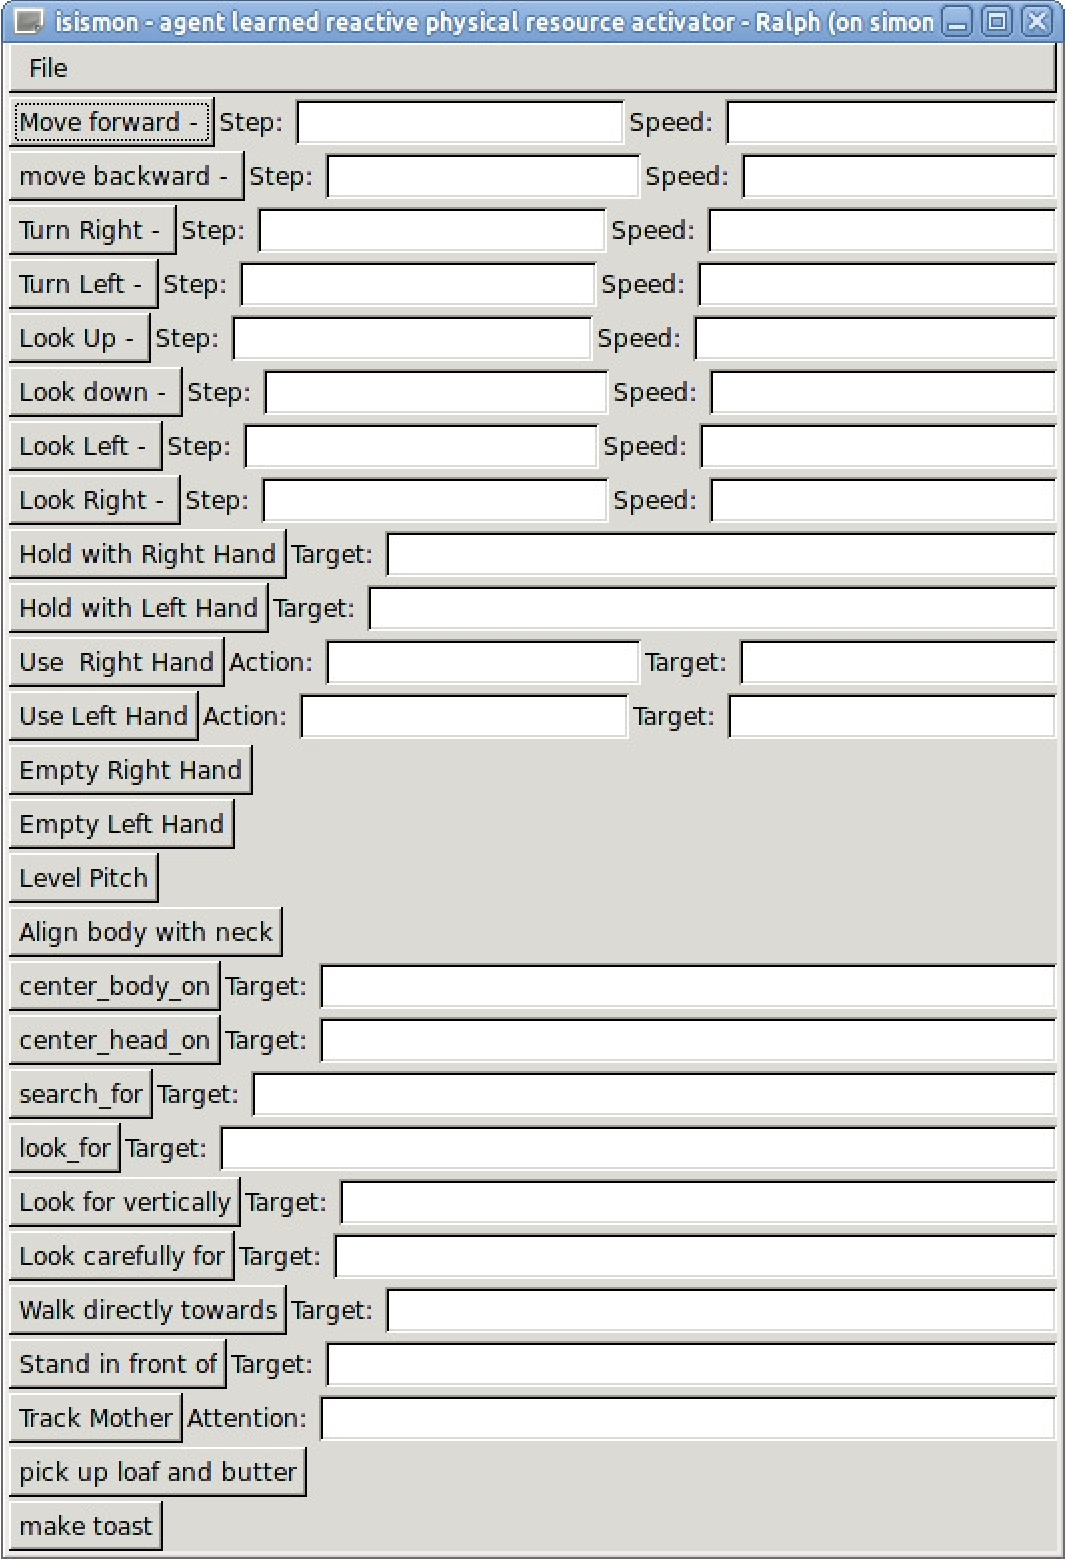
\includegraphics[width=10cm]{gfx/implemented_isisworld_first_order_resource_activator}
%\caption[The implemented semantic event knowledge base.]{The
%  implemented semantic event knowledge base.}
%\label{figure:implemented_isisworld_first_order_resource_activator}
%\end{figure}


\section{First-order Resource Activator}

{\mbox{\autoref{figure:implemented_first_order_resource_activator}}}
shows the implemented first-order resource activator.
\begin{figure}
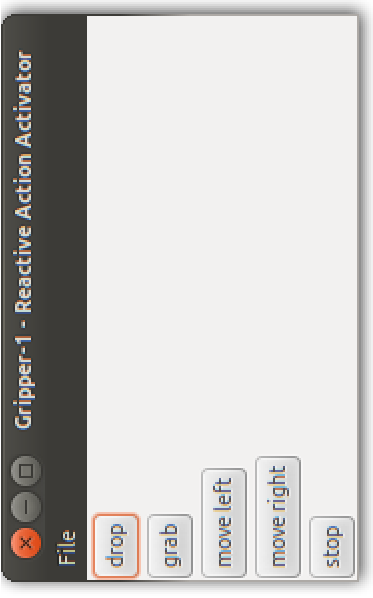
\includegraphics[width=10cm]{gfx/implemented_first_order_resource_activator}
\caption[The implemented first-order resource activator.]{The
  implemented first-order resource activator.}
\label{figure:implemented_first_order_resource_activator}
\end{figure}

\section{First-order Planning Machine Knowledge}

{\mbox{\autoref{figure:implemented_planning_machine_knowledge}}} shows
the implemented first-order planning machine knowledge.
\begin{figure}
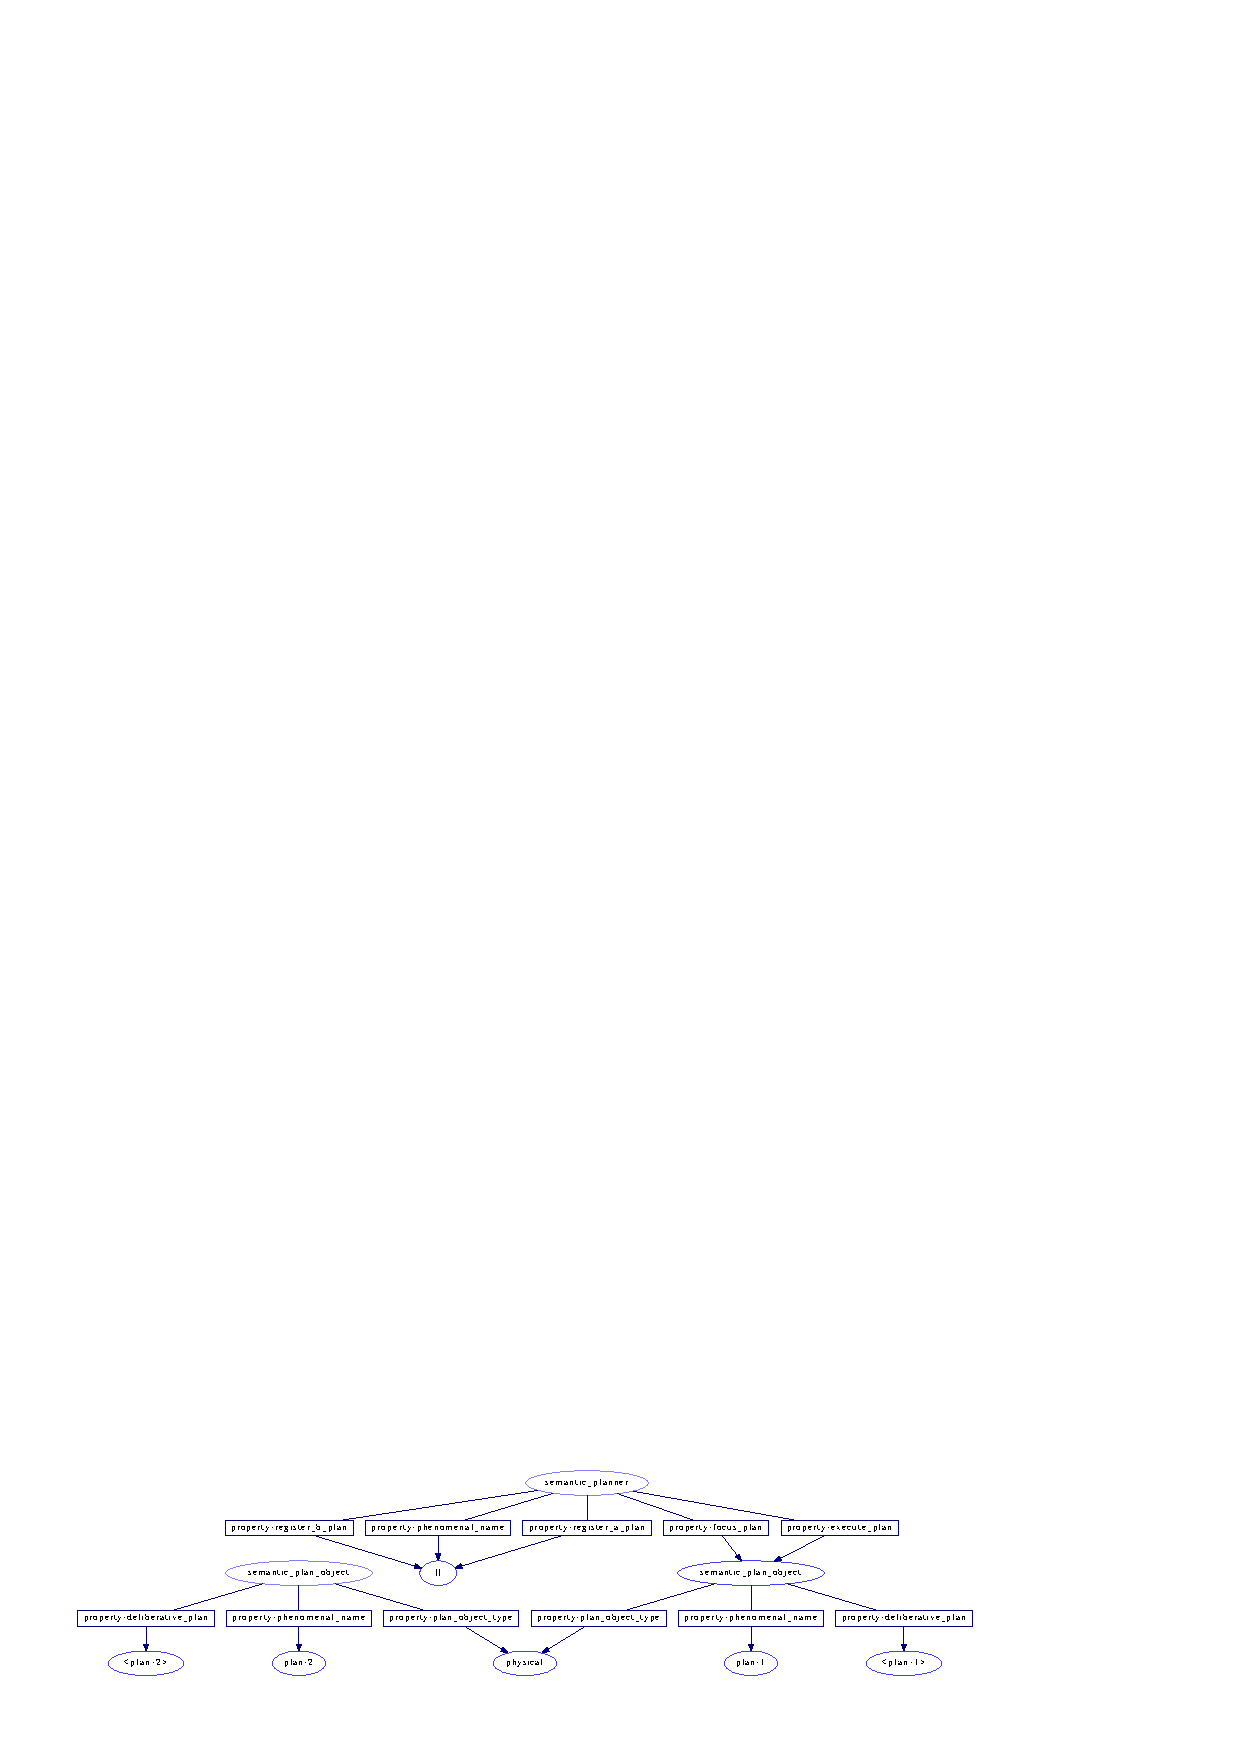
\includegraphics[width=10cm]{gfx/implemented_planning_machine_knowledge}
\caption[The implemented first-order planning machine knowledge.]{The
  implemented first-order planning machine knowledge.}
\label{figure:implemented_first_order_planning_machine_knowledge}
\end{figure}

\section{First-order Plan Activator}

{\mbox{\autoref{figure:implemented_first_order_plan_activator}}} shows
the implemented first-order plan activator.
\begin{figure}
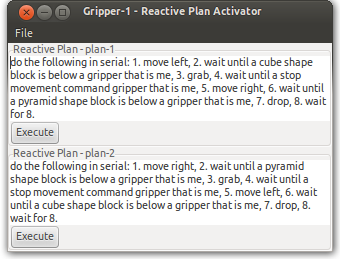
\includegraphics[width=10cm]{gfx/implemented_first_order_plan_activator}
\caption[The implemented first-order plan activator.]{The implemented
  first-order plan activator.}
\label{figure:implemented_first_order_plan_activator}
\end{figure}

\section{Second-order Resource Activator}

{\mbox{\autoref{figure:implemented_second_order_resource_activator}}}
shows the implemented second-order resource activator.
\begin{figure}
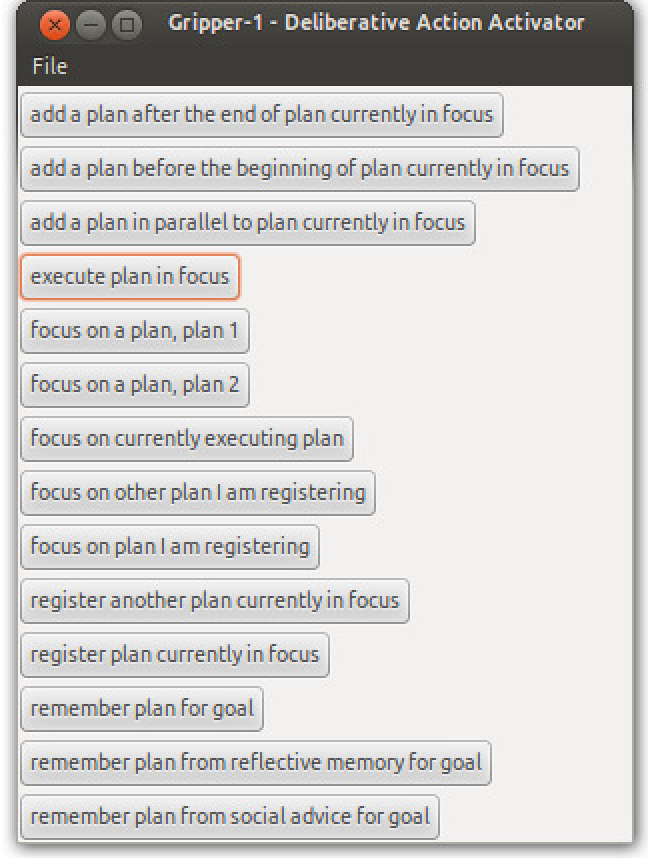
\includegraphics[width=10cm]{gfx/implemented_second_order_resource_activator}
\caption[The implemented second-order resource activator.]{The
  implemented second-order resource activator.}
\label{figure:implemented_second_order_resource_activator}
\end{figure}

